\section{DISCUSSÃO}

\subsection{Por Que a Estratégia Cíclica Supera a Bagging com Warm Start}

O resultado mais marcante deste trabalho --- a superioridade da estratégia Cíclica por uma margem de 9--10 p.p. em TPR --- tem uma explicação arquitetural que se torna ainda mais evidente com 50 rodadas. Ambas as estratégias utilizam \textit{warm start}: cada rodada parte do modelo treinado na rodada anterior, acumulando árvores progressivamente. A diferença está no que acontece com esse modelo acumulado quando múltiplos clientes treinam a partir do mesmo ponto de partida.

Na estratégia Bagging, todos os clientes recebem o mesmo modelo global e treinam independentemente por 25 épocas locais, gerando três versões divergentes do modelo. O servidor seleciona a melhor delas e a envia na próxima rodada --- mas descarta os modelos dos outros dois clientes. Este processo tem um efeito cumulativo: a cada rodada, o modelo global cresce em tamanho (mais árvores), mas parte desse crescimento foi "explorada" por clientes que não foram selecionados, e o modelo escolhido reflete apenas o viés do melhor cliente naquela rodada. Com 50 rodadas e 25 épocas locais, o modelo acumula um número elevado de árvores para um conjunto de dados relativamente pequeno por cliente (264.893 amostras), levando ao sobreajuste clássico de ensemble --- descrito na literatura de boosting como \textit{over-boosting} \cite{chen2016xgboost, ke2017lightgbm}, onde árvores adicionadas além do ponto ótimo começam a memorizar ruído em vez de padrões generalizáveis. O resultado é exatamente o padrão observado na Tabela \ref{tab:convergencia}: pico por volta da rodada 10, seguido de degradação progressiva de 3--5 p.p. até a rodada 50.

Na estratégia Cíclica, o modelo percorre os clientes em sequência --- cada cliente refina o mesmo modelo antes de passá-lo ao próximo, e o ciclo completo equivale a uma rodada efetiva de aprendizado colaborativo. Este mecanismo tem dois efeitos benéficos: primeiro, cada cliente contribui incrementalmente sem descartar o que os outros aprenderam, criando um modelo coeso que integra progressivamente o conhecimento de todos; segundo, o número de árvores adicionadas por ciclo completo é controlado (25 épocas por cliente $\times$ 3 clientes = contribuição distribuída), evitando o crescimento explosivo que ocorre quando um único cliente "vence" a rodada na Bagging. A estabilidade observada da rodada 15 em diante nos três modelos Cíclicos --- com oscilações inferiores a 0,5 p.p. ao longo de 35 rodadas --- confirma que o modelo atingiu um ponto de equilíbrio entre capacidade preditiva e generalização, consistente com o comportamento esperado de modelos de boosting em treinamento sequencial federado \cite{li2020practical}.

\subsection{Comportamento por Algoritmo}

Os três algoritmos mostraram performances notavelmente similares na estratégia Cíclica (55,18--55,88\% TPR, AUC 0,888--0,891), o que reforça que a estratégia de agregação é o fator dominante de desempenho neste cenário, não a escolha do algoritmo em si. As diferenças entre algoritmos na Cíclica são de apenas 0,7 p.p. em TPR e 0,003 em AUC, dentro da margem de variação esperada para uma única execução com semente fixa. No entanto, o CatBoost destacou-se em duas dimensões: apresentou a convergência mais rápida (estabilizando já na rodada 15, enquanto XGBoost e LightGBM ainda mostravam leves oscilações até a rodada 30) e, de longe, o melhor perfil de eficiência (104 segundos, 129 MB). A razão para a eficiência do CatBoost reside em duas características estruturais: o uso de \textit{árvores simétricas} (\textit{oblivious trees}), que aplicam a mesma condição de divisão em todos os nós de um mesmo nível e permitem predições muito mais rápidas por vetorização, e o tratamento nativo de variáveis categóricas, que elimina etapas de pré-processamento custosas \cite{prokhorenkova2018catboost}. Vale notar que o \textit{ordered boosting} --- outra técnica característica do CatBoost --- não está relacionado à velocidade: seu propósito é evitar um viés de estimação do gradiente presente em outros algoritmos de boosting, podendo inclusive aumentar o custo computacional em certos cenários \cite{prokhorenkova2018catboost}. Na estratégia Bagging, o LightGBM foi o mais penalizado (2.573 segundos, 1.028 MB), pois a estratégia de agregação por ensemble de todos os clientes paralelamente amplifica o custo do LightGBM por ter o maior número de estimadores (276 por rodada).

\subsection{O Mecanismo de Correção de Fairness}

O ajuste de fairness implementado neste trabalho utiliza a técnica de \textit{post-processing} com limiares de decisão específicos por grupo demográfico, sem modificar o modelo treinado \cite{hardt2016equality}. No regime \textbf{standard}, um único limiar $\tau$ é calibrado no conjunto completo para que a taxa de falsos positivos global seja exatamente 5\%. No regime \textbf{fair}, dois limiares independentes são calibrados: $\tau_{\text{jovem}}$ para o grupo idade $< 50$ e $\tau_{\text{idoso}}$ para o grupo idade $\geq 50$, cada um ajustado para que o FPR do respectivo grupo seja 5\%. A decisão passa a ser:
\[
\hat{y} = \begin{cases}
\mathds{1}[p(x) \geq \tau_{\text{jovem}}] & \text{se~idade} < 50 \\
\mathds{1}[p(x) \geq \tau_{\text{idoso}}] & \text{se~idade} \geq 50
\end{cases}
\]
Esta abordagem equaliza as taxas de falso positivo entre grupos (equalized odds de FPR \cite{hardt2016equality}) sem exigir acesso aos dados originais de outros clientes e sem alterar o treinamento federado --- propriedades importantes em cenários de privacidade. O custo observado foi moderado: perda média de 1,7--2,0 p.p. em TPR para todos os modelos Cíclicos, elevando o FPR Ratio de 0,28--0,29 para 0,97--1,00. O resultado é especialmente relevante para o XGBoost Cíclico, que no regime fair alcançou FPR Ratio de 0,999 --- na prática, as taxas de falso positivo entre jovens e idosos são estatisticamente indistinguíveis --- com TPR de 53,08\%.

\subsection{Trade-off Fairness--Desempenho}

A análise conjunta dos dois regimes de limiar revela um \textit{trade-off} controlável e favorável: a equalização de fairness custa, em média, menos de 2 p.p. em TPR para as configurações Cíclicas. Este resultado é consistente com estudos de fairness em modelos de detecção de fraude que indicam que a calibração de limiares por grupo tende a ser mais eficiente em termos de custo de desempenho do que abordagens aplicadas durante o treinamento do modelo \cite{hardt2016equality}. Em termos práticos, o regime fair viabiliza conformidade com requisitos regulatórios de não-discriminação \cite{gdpr2016} com impacto limitado na capacidade de detecção: uma perda de $\approx$ 2 p.p. em TPR significa que, a cada 10.000 fraudes, cerca de 200 a mais escapariam à detecção em troca de garantir que clientes legítimos de diferentes faixas etárias sejam afetados igualitariamente por falsos alertas. Este balanço é uma decisão de negócio e regulatória, mas os resultados mostram que ele é factível tecnicamente.

A Figura~\ref{fig:tradeoff} oferece uma perspectiva geométrica desse trade-off: cada modelo é posicionado no espaço definido pelo eixo horizontal (FPR Ratio, quanto mais próximo de 1,0 mais equitativo) e pelo eixo vertical (TPR@5\%FPR, quanto maior melhor). Círculos representam o regime Standard e quadrados o regime Fair. A leitura do gráfico revela três padrões sobrepostos. Primeiro, a separação vertical entre os dois grupos de estratégias é absoluta --- todos os modelos Cíclicos estão acima de todos os Bagging, confirmando que a estratégia de agregação domina o eixo de desempenho. Segundo, a transição do regime Standard para o Fair provoca em todos os modelos um deslocamento para a direita (FPR Ratio melhora) com queda modesta no eixo vertical (TPR cai levemente), o que geometricamente corresponde a um deslocamento diagonal favorável dentro da região de alta equidade (área sombreada em verde). Terceiro, os modelos Cíclicos no regime Fair concentram-se no quadrante superior direito --- alta TPR \textit{e} alta equidade simultaneamente --- enquanto os modelos Bagging, mesmo após a correção Fair, permanecem no quadrante inferior direito, com boa equidade mas TPR insuficiente. O XGBoost Cíclico Fair destaca-se como o ponto mais à direita do grupo de melhor desempenho, com FPR Ratio de 0,999 e TPR de 53,08\% --- virtualmente no cruzamento entre as linhas de fairness ideal e teto do baseline centralizado.

\begin{figure}[H]
\centering
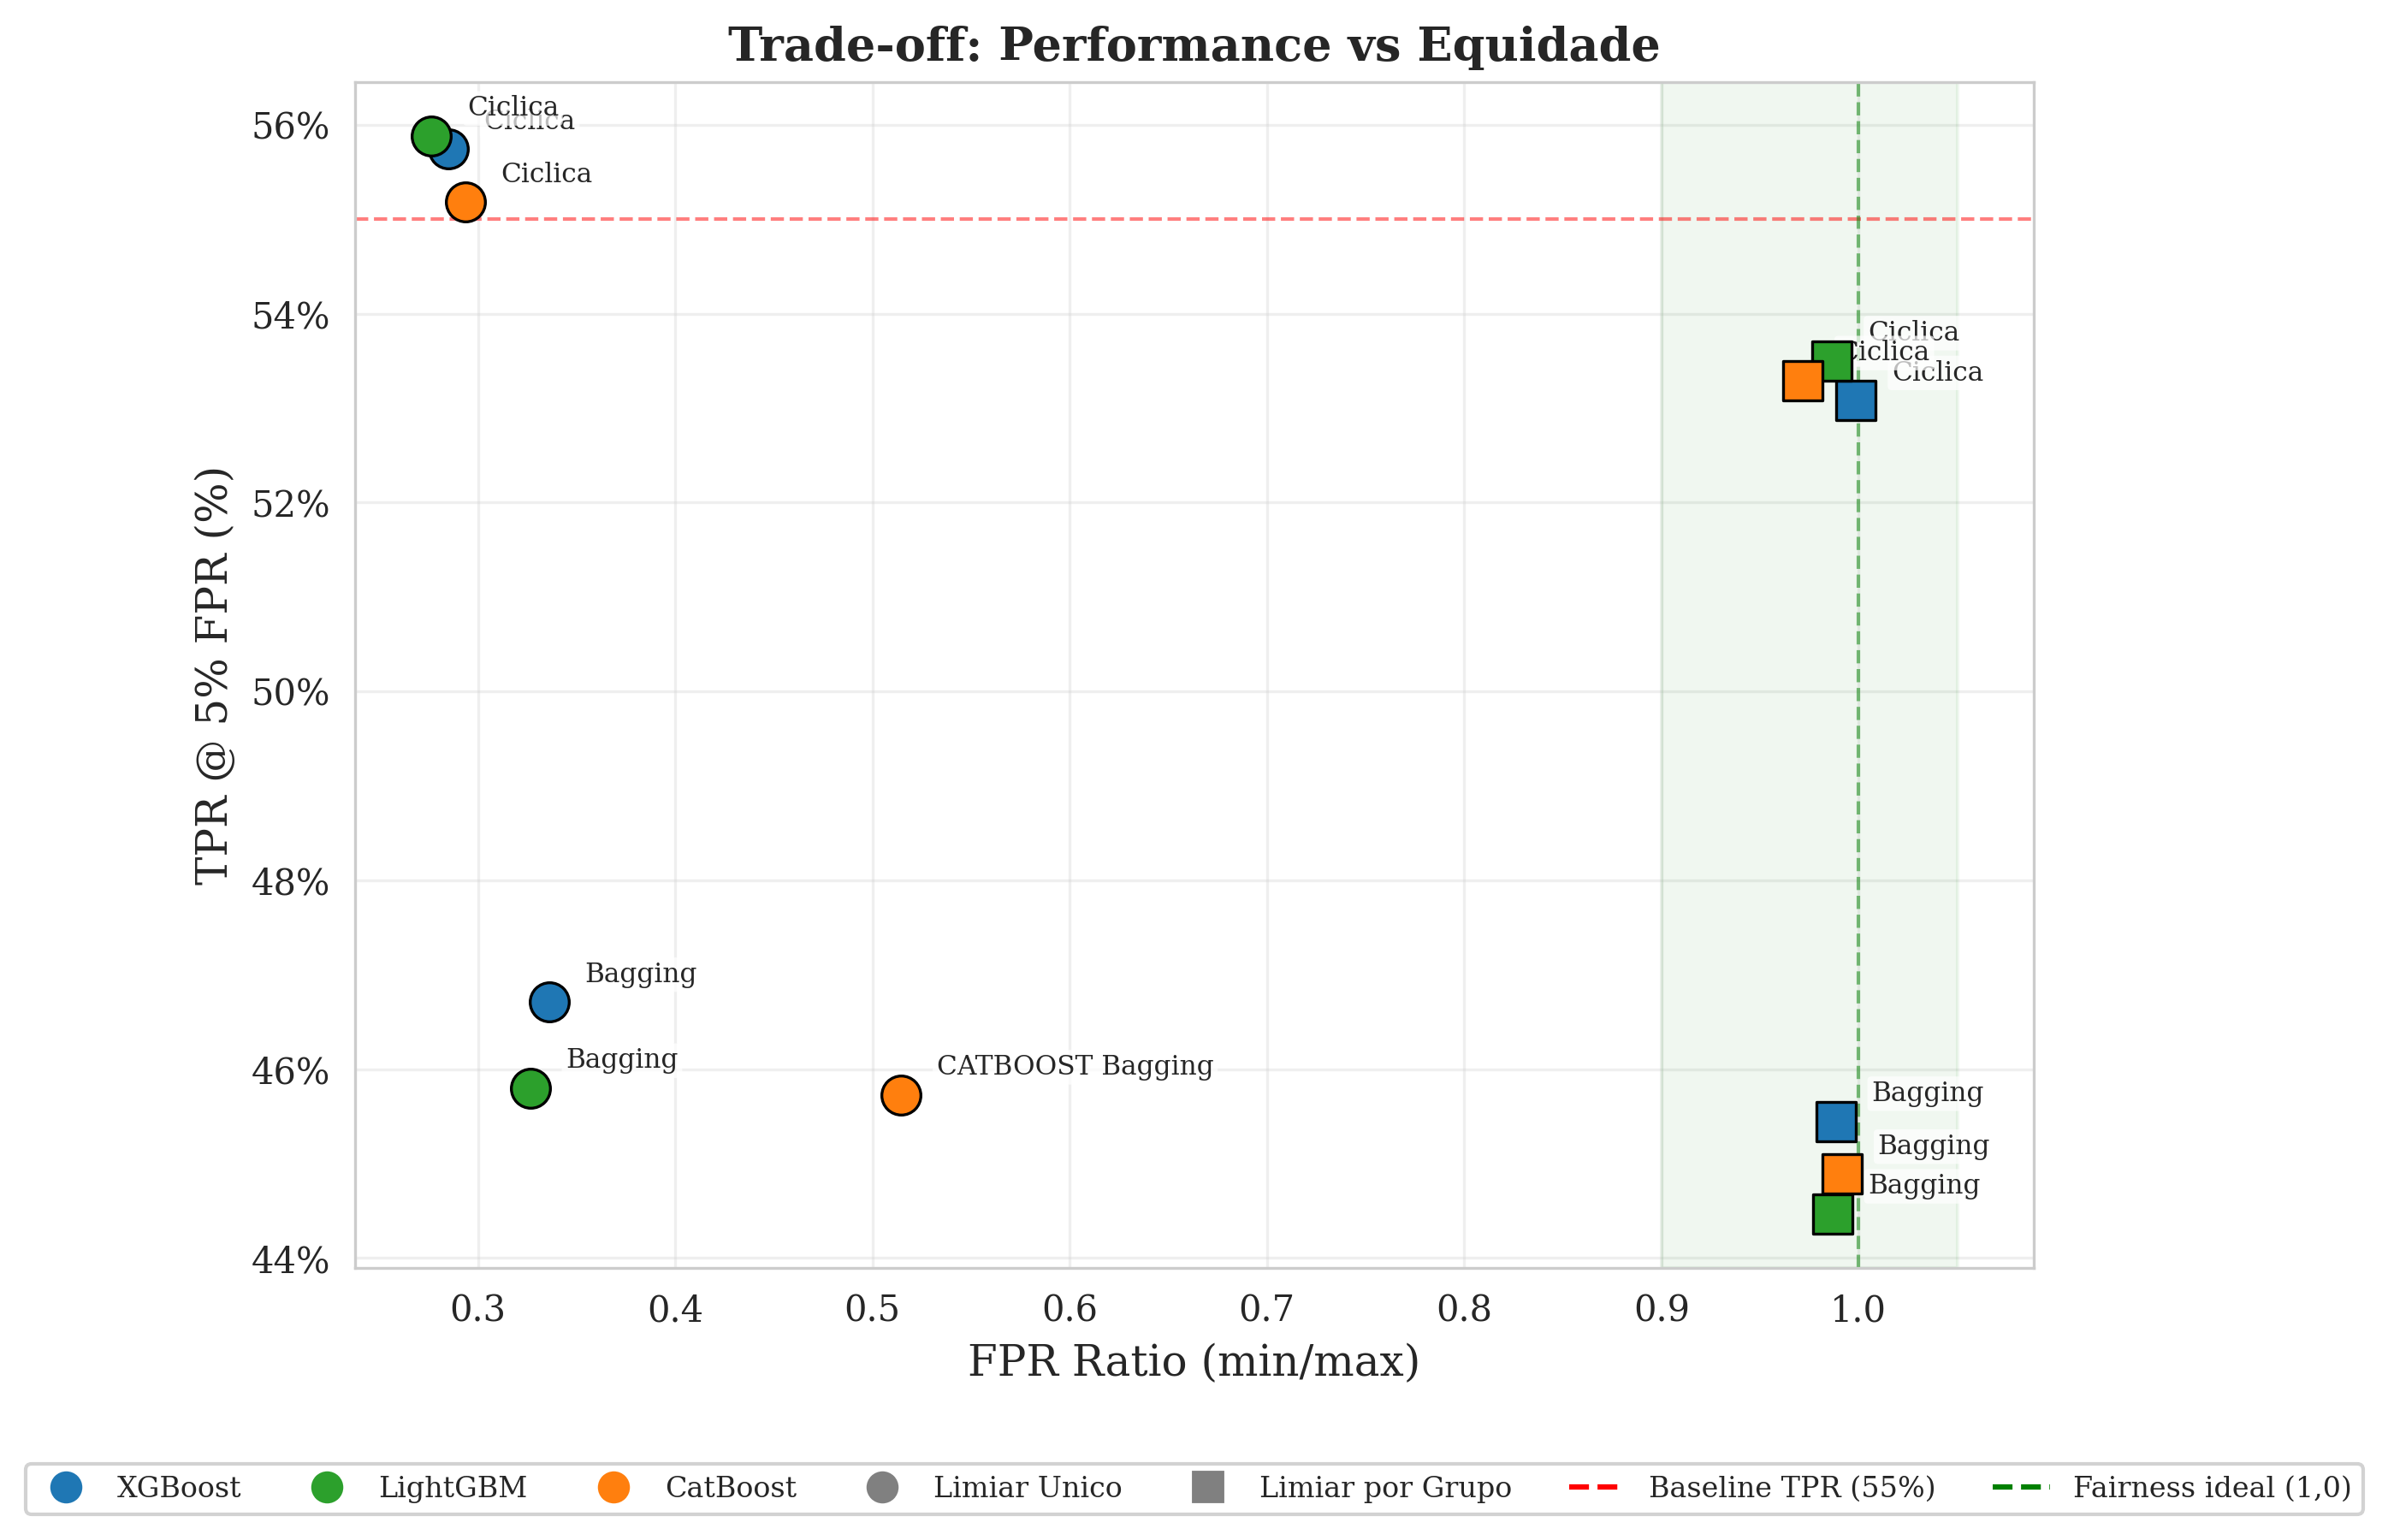
\includegraphics[width=0.82\textwidth]{figures/plots_originais/tradeoff_performance_fairness.png}
\caption{Trade-off entre desempenho (TPR@5\%FPR, eixo vertical) e equidade demográfica (FPR Ratio, eixo horizontal) para todas as configurações, nos dois regimes de limiar. Círculos: regime Standard; quadrados: regime Fair. Linha vermelha tracejada: teto do \textit{baseline} centralizado (55\%); linha verde tracejada: fairness ideal (FPR Ratio = 1,0); região sombreada verde: zona de alta equidade (FPR Ratio $\geq 0,9$). O quadrante superior direito é a região de maior desempenho e maior equidade simultâneos, ocupado exclusivamente pelos modelos Cíclicos no regime Fair.}
\label{fig:tradeoff}
\end{figure}

\subsection{Desafios de Implementação}

Vários desafios técnicos foram identificados e resolvidos durante o desenvolvimento, e seu registro é relevante tanto para reprodutibilidade quanto para orientar implementações futuras.

\textbf{Serialização heterogênea de modelos.} A transmissão de modelos entre clientes e servidor requer serialização em bytes, mas cada framework possui uma API distinta: o XGBoost permite serialização direta em JSON via \texttt{save\_raw()}, enquanto LightGBM e CatBoost exigem gravação em arquivos temporários. Para unificar o processo, foi adotada uma abordagem baseada em \textit{pickle} com arrays NumPy, garantindo compatibilidade entre os três algoritmos e o protocolo de comunicação do Flower.

\textbf{Crescimento do modelo com warm start.} O \textit{warm start} acumula árvores a cada rodada, o que implica crescimento linear do modelo transmitido. Com 50 rodadas e 25 épocas locais, o tamanho dos modelos ao final do experimento é substancialmente maior do que na rodada inicial, conforme evidenciado pelo volume de comunicação crescente observado na Tabela \ref{tab:eficiencia}. Em cenários com muito mais rodadas ou clientes, técnicas de poda de árvores (\textit{pruning}) ou limitação do número máximo de estimadores seriam necessárias para controlar o crescimento do modelo.

\textbf{Desbalanceamento severo de classes.} A taxa de fraude de apenas 1,03\% no treinamento exige mecanismos específicos para evitar que o modelo trivialmente classifique tudo como legítimo. A solução adotada foi o parâmetro nativo de pesos de classe (\texttt{scale\_pos\_weight} para XGBoost e LightGBM, \texttt{auto\_class\_weights='Balanced'} para CatBoost), compatível com o particionamento federado pois não exige acesso a dados de outros clientes, ao contrário de técnicas de sobreamostragem (como SMOTE) que exigiriam acesso aos dados de outros clientes.

\textbf{Otimização federada de hiperparâmetros.} A execução do Optuna independentemente em cada cliente, com 50 \textit{trials} por cliente e 33\% dos dados locais, foi eficaz em encontrar hiperparâmetros de boa qualidade. A agregação via mediana mostrou-se robusta: os três clientes, com distribuições de dados idênticas (IID), produziram configurações similares, resultando em medianas estáveis. Em cenários Non-IID, esta etapa poderia gerar configurações mais divergentes entre clientes, exigindo abordagens de agregação mais sofisticadas.

\subsection{Limitações do Trabalho}

Os resultados devem ser interpretados dentro das limitações do experimento. O particionamento IID balanceado, embora conveniente para isolar o efeito das estratégias de agregação, não captura a heterogeneidade estatística presente em cenários reais onde diferentes instituições financeiras possuem perfis de clientes distintos \cite{zhu2021noniid}; cenários Non-IID tendem a prejudicar mais fortemente a estratégia Cíclica, que depende da coerência semântica entre os modelos sequencialmente refinados pelos clientes. A simulação com apenas 3 clientes também limita as conclusões de escalabilidade: com dezenas de participantes, a estratégia Cíclica pode se tornar proibitivamente lenta (a latência de cada rodada é proporcional ao número de clientes), enquanto a Bagging mantém latência aproximadamente constante por paralelizar o treinamento \cite{bonawitz2019scale}. As execuções foram realizadas uma única vez com semente fixa (\texttt{seed=42}), sem repetições para estimativa de variância estatística, o que limita a interpretação de diferenças pequenas entre algoritmos. Por fim, o sistema não implementa mecanismos de privacidade como Agregação Segura \cite{bonawitz2017secagg} ou Privacidade Diferencial \cite{geyer2017differential}, focando exclusivamente na avaliação de desempenho e fairness dos algoritmos no contexto federado.

\subsection{Implicações Práticas}

Os resultados sugerem recomendações concretas para sistemas federados de detecção de fraude bancária. Para cenários que priorizam desempenho com restrição de comunicação, o \textbf{CatBoost Cíclico com regime fair} oferece o melhor equilíbrio: TPR de 53,29\%, FPR Ratio de 0,972, 104 segundos por experimento completo e apenas 129 MB de dados transferidos em 50 rodadas --- e boa parte desse desempenho está disponível já nas rodadas 15--20, sugerindo que em produção 20 rodadas seriam suficientes com redução proporcional de custo. Para cenários que priorizam fairness máxima, o \textbf{XGBoost Cíclico com regime fair} alcança FPR Ratio de 0,999 com TPR de 53,08\%. A estratégia Bagging não é recomendada para boosting federado com \textit{warm start} em cenários com muitas rodadas, pois a degradação observada --- consistente com o fenômeno de \textit{over-boosting} na literatura \cite{chen2016xgboost} --- anula os ganhos iniciais. Se a Bagging for necessária (por exemplo, em cenários Non-IID onde o ensemble de modelos heterogêneos pode ser vantajoso), deveria ser utilizada com um número reduzido de rodadas (5--10) antes que a degradação se instale. A baixa transferência de dados dos modelos de árvore (129--1.028 MB em 50 rodadas, reduzindo para 26--205 MB com 10 rodadas) é compatível com redes de largura de banda limitada, confirmando a vantagem sobre redes neurais profundas que transmitem o mesmo volume independentemente do número de rodadas \cite{konecny2016communication, liu2024survey}.
